\section{Achszähler}\label{text:Entwicklung-der-GFA:Achszähler}

In diesem Abschnitt wird die Entwicklung der Achszähler beschrieben. Die Achszähler sind die Grundlage für die Gleisfreimeldeanlage und dienen dazu, die Position der Züge auf der Anlage zu bestimmen. Die Achszähler bestehen aus einem Mikrocontroller, welcher die Sensoren auswertet und die Anzahl der Achsen zählt. Zunächst werden die in \autoref{text:Methodik:Achszähler} \nameref{text:Methodik:Achszähler} vorgestellten Möglichkeiten zur Realisierung eines Achszählers betrachtet und die Entscheidung für eine der Methoden getroffen. Anschließend wird die Umsetzung des Achszählers beschrieben.

\subsection{Sensor-Tests}\label{text:Entwicklung-der-GFA:Achszähler:Sensor-Tests}

Zur Entscheidungsfindung, welcher Sensor für die Realisierung des Achszählers verwendet wird, wurden Tests mit den in \autoref{text:Methodik:Achszähler} \nameref{text:Methodik:Achszähler} vorgestellten Sensoren durchgeführt. Die Tests wurden abstrakt auf einem Steckbrett durchgeführt, um die Funktionen in verschiedenen Szenarien zu testen.

\subsubsection{IR-Lichtschranke}\label{text:Entwicklung-der-GFA:Achszähler:Sensor-Tests:Lichtschranke}

Für die Tests der IR-Lichtschranke wurde eine Infrarot-LED und ein Fototransistor verwendet. Die LED wurde mit einem Vorwiderstand an eine Spannungsquelle angeschlossen und der Fototransistor an eine LED um die Funktion zu visualisieren. Die Schaltung ist in \autoref{abb:IR-Lichtschranke} dargestellt. Die LED leuchtet, solange der Fototransistor angestrahlt wird. Wird der Fototransistor durch ein Objekt verdeckt, leuchtet die LED nicht mehr.

\begin{figure}[H]
    \centering
    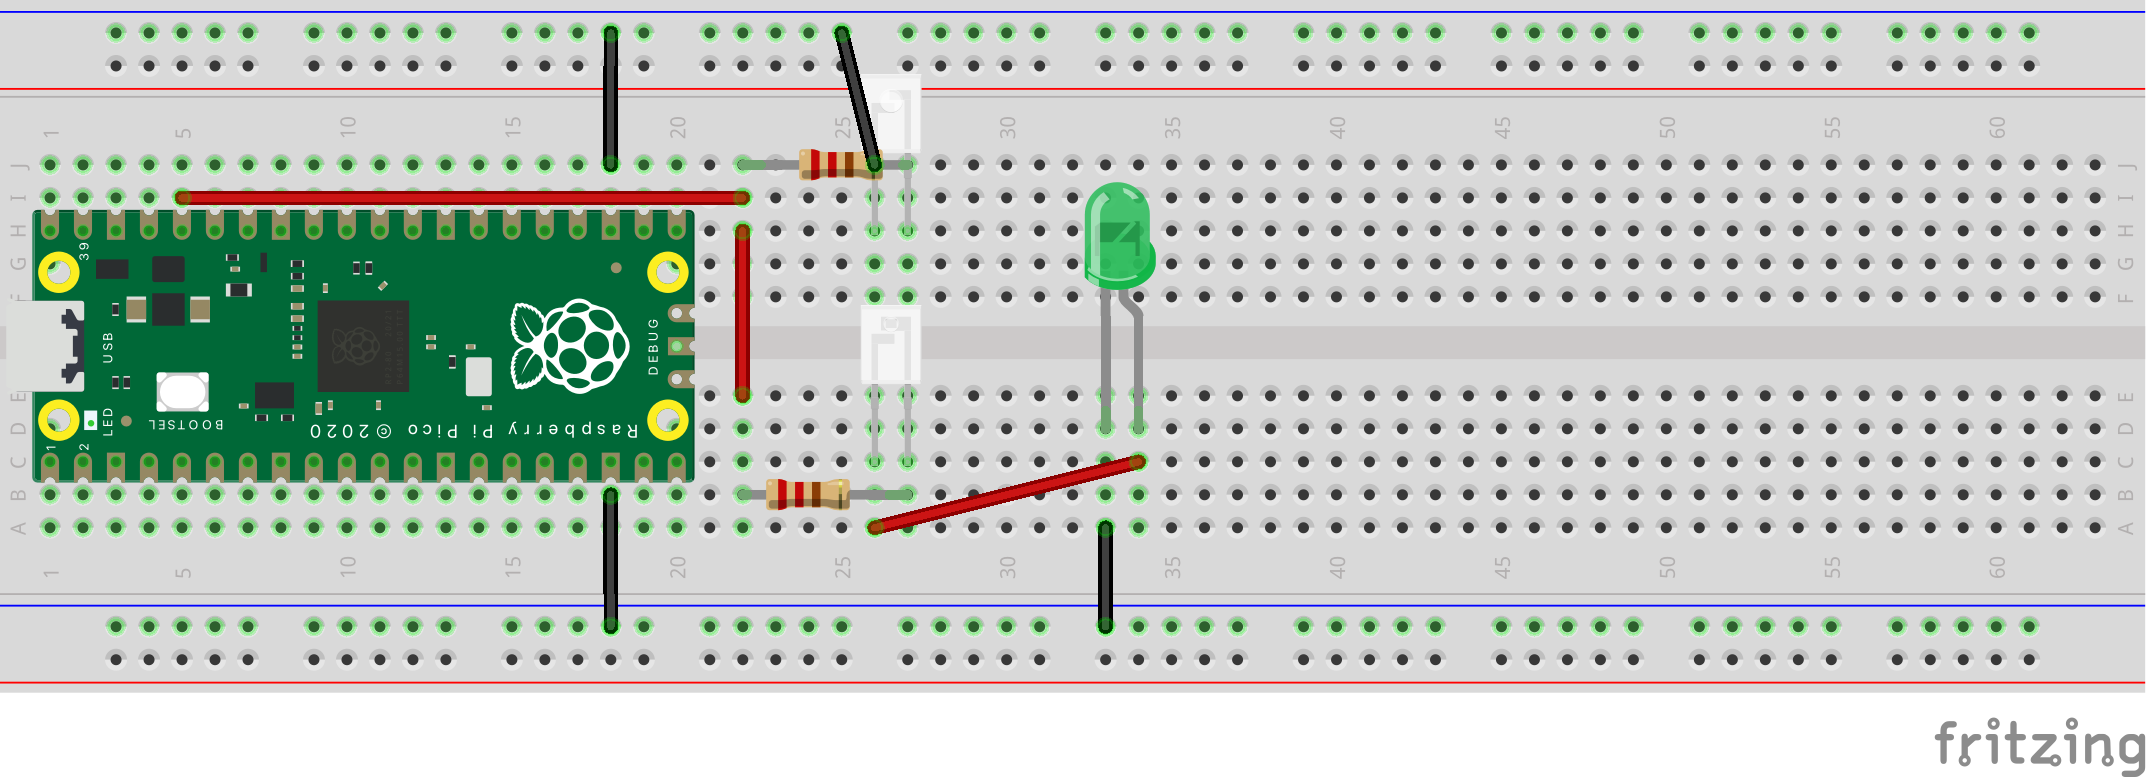
\includegraphics[width=0.7\textwidth]{Assets/Images/4-Entwicklung-der-GFA/IR-Test_bb.png}
    \caption{Testaufbau der IR-Lichtschranke}\label{abb:IR-Lichtschranke}
\end{figure}

Die Funktion der Lichtschranke wurde mit folgenden Szenarien jeweils bei indirekter, direkter und keiner Beleuchtung getestet:

\begin{itemize}
    \item Die Lichtschranke wird von einem Objekt durchfahren.
    \item Die Lichtschranke wird von einem Objekt durchfahren, welches sich langsam bewegt.
    \item Die Lichtschranke wird von einem Objekt durchfahren, welches sich schnell bewegt.
    \item Die Lichtschranke wird von mehreren Objekten mit geringen Abständen durchfahren.
\end{itemize}

Die Tests ergaben, dass die Infrarot-Lichtschranke unter allen Bedingungen zuverlässig funktioniert. Die Lichtschranke kann auch bei direkter Sonneneinstrahlung und bei Dunkelheit zuverlässig betrieben werden. Dementsprechend ist die Lichtschranke für die Realisierung des Achszählers geeignet.

\subsubsection{Hall-Sensor}\label{text:Entwicklung-der-GFA:Achszähler:Sensor-Tests:Hall-Sensor}

Der Hall-Sensor konnte aus zeitlichen Gründen nicht getestet werden, da die Entscheidung aus Kosten- und Inventar-Gründen bereits gefallen war. Der Hall-Sensor ist jedoch für die Realisierung des Achszählers geeignet, sofern die Fahrzeuge mit einem oder mehreren Magneten ausgestattet werden. Das einzige Problem, welches bei der Verwendung von Hall-Sensoren auftreten kann, ist der zu geringe Abstand zwischen Magneten, wodurch die Sensoren eventuell nicht zuverlässig auslösen und eine \"Dauerüberfahrt\" detektieren. Die einzuhaltenden Abstände konnten aus oben genannten Gründen nicht getestet werden.

\subsubsection{Reed-Kontakt}\label{text:Entwicklung-der-GFA:Achszähler:Sensor-Tests:Reed-Kontakt}

Für die Tests des Reed-Kontakts wurde ein solcher Kontakt, ein Magnet und eine LED verwendet. Der Reed-Kontakt, welcher als Schalter fungiert, schließt sich, wenn ein Magnet in die Nähe des Kontakts gebracht wird. Die Schaltung ist in \autoref{abb:Reed-Kontakt} dargestellt. Die LED leuchtet, solange der Reed-Kontakt geschlossen ist. Wird der Magnet entfernt, öffnet sich der Kontakt und die LED leuchtet nicht mehr.

\begin{figure}[H]
    \centering
    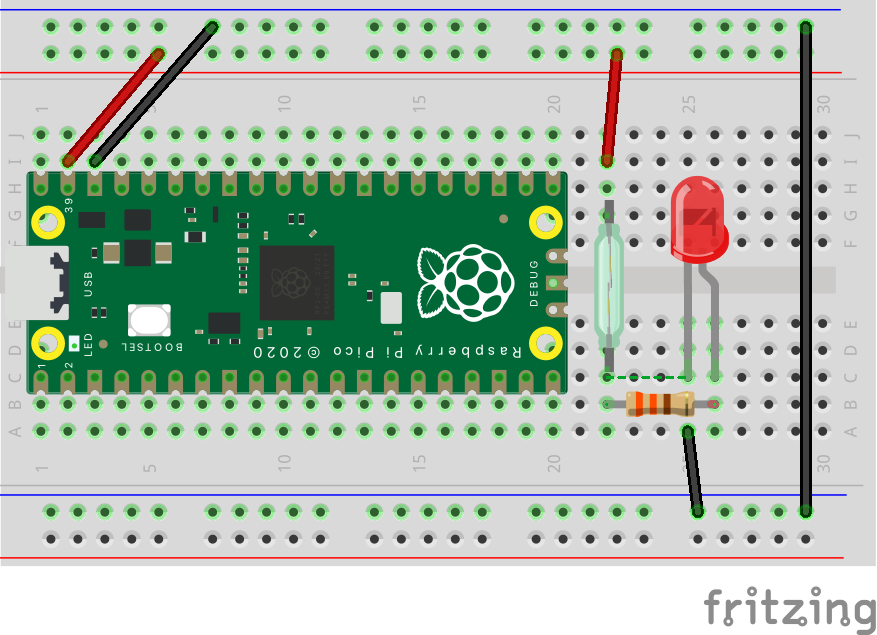
\includegraphics[width=0.7\textwidth]{Assets/Images/4-Entwicklung-der-GFA/Reed-Test1_bb.png}
    \caption{Testaufbau des Reed-Kontakts}\label{abb:Reed-Kontakt}
\end{figure}

Durch die Tests konnte festgestellt werden, dass der Reed-Kontakt zuverlässig funktioniert, solange der Magnet mit einem Abstand von maximal 1 cm an den Kontakt gebracht wird. Zusätzlich wurde der Sensor mit einem Magneten getestet, welcher wie in \autoref{abb:Magnet} dargestellt, in einem Klemmbaustein befestigt wurde. Der Klemmbaustein scheint die Funktion des Reed-Kontakts nicht zu beeinflussen.

\begin{figure}[H]
    \centering
    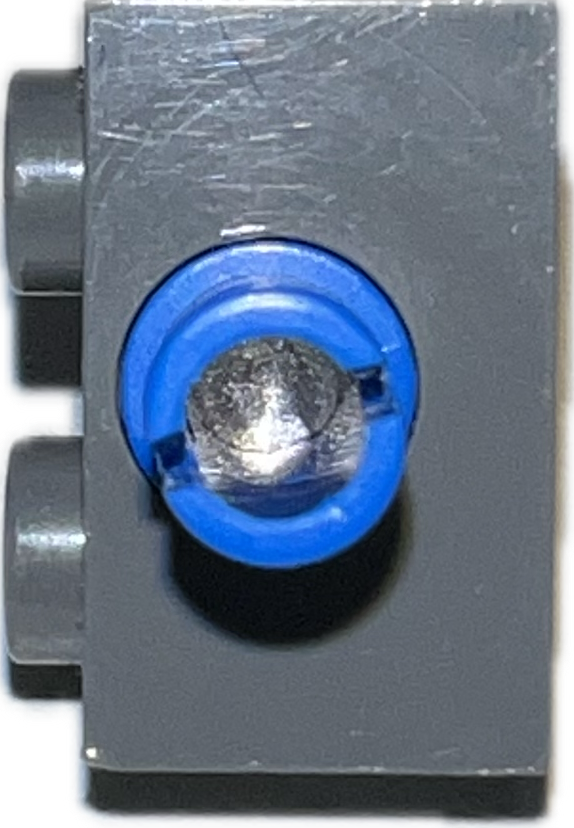
\includegraphics[width=0.35\textwidth]{Assets/Images/4-Entwicklung-der-GFA/Magnet.png}
    \caption{Testaufbau des Reed-Kontakts mit Klemmbaustein}\label{abb:Magnet}
\end{figure}

\subsection{Entscheidung}\label{text:Entwicklung-der-GFA:Achszähler:Entscheidung}

Die Tests der Sensoren haben ergeben, dass sowohl die IR-Lichtschranke als auch der Reed-Kontakt zuverlässig funktionieren und für den Achszähler verwendet werden können. Der Hall-Sensor wurde aufgrund von Zeitmangel nicht getestet, ist jedoch ebenfalls für den Achszähler geeignet. Da die IR-Lichtschranke und der Reed-Kontakt bereits vorhanden sind, wurde entschieden, den Achszähler mit einem Reed-Kontakt zu realisieren.
\newline
Gründe für die Entscheidung des Reed-Kontakts sind die geringen Kosten und die einfache Handhabung und Wartbarkeit. Außerdem kommt eine Lösung welche mit Hilfe von Magnetfeldern funktioniert näher an die Realität heran. Die Reed-Kontakte können diskreter direkt in das Gleisbett verbaut werden und sind nicht so offensichtlich eintlang der Strecke sichtbar.
